\documentclass[aspectratio=169,xetex,compress,xcolor={table}]{beamer}
\usepackage{nectec}

\title{\bfseries \LARGE Free \& Open Source Software}
\subtitle{\normalfont \large \slshape เพื่อลดปัญหาการละเมิดลิขสิทธิ์}
\author{\bfseries ศุภโชค ศันติวิชยะ}
\institute{\slshape งานยกระดับความพร้อมทางเทคโนโลยี ฝ่ายสนับสนุนบริการทางวิศวกรรมและเทคโนโลยี \\
ศูนย์อิเล็กทรอนิกส์และตอมพิวเตอร์แห่งชาติ\\
สำนักงานพัฒนาวิทยาศาสตร์และเทคโนโลยีแห่งชาติ}
\date{\printdate{2021}{4}{8}}
% \logo{
\includegraphics[height=0.5cm]{nectec.png}}
\mode<presentation>

\begin{document}

% Title
{
\beamertemplatenavigationsymbolsempty %
\setbeamertemplate{headline}{\vspace{13.2mm}}
\coverbg
\frame{\titlepage}
}

% Outline

\setbeamertemplate{section in toc}[ball unnumbered]
\section*{Outlines}
\begin{frame}[t]
  \frametitle{Outline}
  \tableofcontents[hidesubsections]
\end{frame}

% Frams

\section{Free \& Open Source Software}
\subsection{FOSS}
% !TeX root = ../.tex

\begin{frame}
  \frametitle{Free \& Open Source Software}
  \begin{columns}

    \column{0.4\textwidth}
    \begin{center}
      
\includegraphics[width=.7\linewidth]{images/foss-logo.png}
    \end{center}

    \column{0.6\textwidth}
    \begin{beamerboxesrounded}[shadow=true,width=.9\textwidth]{\bfseries FOSS}
      \centering \Large \underline{\slshape \bfseries F}ree  %
      \underline{\slshape \bfseries O}pen %
      \underline{\slshape \bfseries S}ource %
      \underline{\slshape \bfseries S}oftware
    \end{beamerboxesrounded}
  \end{columns}

\end{frame}


\subsection{The Free Software Foundation}
% !TeX root = ../.tex

\begin{frame}[t]
  \frametitle{The Free Software Foundation (FSF)\footnotemark[1]}
  \begin{columns}

    \column[c]{0.6\textwidth}
    \textbf{Richard Stoallman}
    \begin{itemize}[<+->]
      \item สร้าง EMACS กับ GNU Project (1984)
      \item ก่อตั้ง Free Software Foundation  (1985)
      \item Free Software (ซอฟต์แวร์เสรี)
      \item ให้คำจำกัดความของเสรีภาพทั้งสี่
    \end{itemize}

    \column{0.4\textwidth}
    \begin{center}
      \includegraphics<1->[width=.7\linewidth]{images/fsf-gnu-logo.png}
    \end{center}
  \end{columns}

  \footnotetext[1]{\url{https://fsf.org}}

\end{frame}
% !TeX root = ../.tex

\begin{frame}[t]
  \frametitle{Four Essential Freedoms \footnotemark[2]}
  \begin{columns}
    \column[c]{0.5\textwidth}
    \begin{center}
      \includegraphics<1>[width=.7\linewidth]{images/0run.png}
      \includegraphics<2>[width=.75\linewidth]{images/1study.png}
      \includegraphics<3>[width=.7\linewidth]{images/2redistribute.png}
      \includegraphics<4>[width=.7\linewidth]{images/3distribute.png}
      \includegraphics<5>[width=.7\linewidth]{images/4freedoms.png}
    \end{center}
    \column[b]{0.5\textwidth}
    \begin{enumerate}
      \setcounter{enumi}{-1}
      \item<1,5> Freedom to RUN
      \item<2,5> Freedom to STUDY
      \item<3,5> Freedom to Redistribute
      \item<4,5> Freedom to Distribute
    \end{enumerate}
  \end{columns}
  \footnotetext[2]{\url{https://www.gnu.org/philosophy/free-sw.en.html}}

\end{frame}

\subsection{Open Source Software}
% !TeX root = ../.tex

\begin{frame}
  \frametitle{Open Source Initiative (OSI) \footnotemark[3]}
  \begin{columns}

    \column[c]{0.6\textwidth}
    \begin{itemize}[<+->]
      \item Eric Raymond is first President (1998)
      \item จดเครื่องหมายการค้า ``Open Source''
      \item กำหนดนิยามของ ``Open Source'' 10 ข้อ
      \item ตรวจสอบรับรอง open source license
      \item ผลักดัน open source เป็นมิตรกับภาคธุรกิจ
      \item The Cathedral and The Bazaar \footnotemark[4]\  \footnotemark[5]
      \item เกิด Mozilla Foundation สร้าง Firefox ตามแนวทาง open source (Netscape)
    \end{itemize}

    \column{0.4\textwidth}
    \begin{center}
      \includegraphics<1->[width=.7\linewidth]{images/osi-logo.png}
    \end{center}
  \end{columns}

  \footnotetext[3]{\url{https://opensource.org}}
  \footnotetext[4]{ต้นฉบับ \url{http://www.catb.org/~esr/writings/cathedral-bazaar/cathedral-bazaar/}}
  \footnotetext[5]{ภาษาไทย \url{https://linux.thai.net/~thep/catb/cathedral-bazaar/}}


\end{frame}
% !TeX root = ../.tex
\begin{frame}
  \frametitle{The Open Source Definition \footnotemark[6]}

  \begin{multicols}{2}
    \begin{enumerate}
      \small
      \item Freely Redistributable
      \item Source Code Included
      \item Derived Works Permitted
      \item Integrity of Author’s Source Code
      \item  No Discrimination Against Persons or Groups
      \item No Discrimination Against Fields of Endeavour
      \item Distribution of Licence (Rights)
      \item Licence Must Not Be Specific to a Product
      \item Licence Must Not Restrict Other Software
      \item Licence Must Be Technology-Neutral
    \end{enumerate}
  \end{multicols}
  \footnotetext[6]{\url{https://opensource.org/osd}}
\end{frame}

\subsection{Definition}
% !TeX root = ../.tex
\begin{frame}
  \frametitle{Defination}
  \begin{center}
    \textbf{\Large
      \shadowbox{ Open Source  Software $\neq$ Free Software }\pause \\
      \alert{Free as freedom} \\
      \emph{(not free of charge)} \pause \\
      Open Source Software (OSS)  \pause \\
      Free and Open Source Software (FOSS) \pause \\
      Free and Libre and Open Source Software  (FLOSS) \\ \pause
      \shadowbox{\alert{ ไม่เกี่ยวกับ Freeware $\&$ Shareware} }
    }
  \end{center}
\end{frame}

\section{ลิขสิทธิ์}
\subsection{License classifications}
% !TeX root = ../.tex
\begin{frame}
  \frametitle{License classifications \footnotemark[11] }
  \resizebox{\linewidth}{!}{
    \rowcolors[]{1}{gray!10}{white}
    \begin{tabular}{lccccccccc} \toprule
      \bfseries License                           & \bfseries CopyLeft      & \bfseries  Permissive  & \bfseries  Linking        &                                                                                      %
      \bfseries  Distribution                     & \bfseries  Modification & \bfseries Patent grant & \bfseries Private use     &                                                                                      %
      \bfseries Sublicensing                      & \bfseries Grants TM                                                                                                                                                 \\ \midrule

      Academic Free License                       &                         & Yes                    & Yes                       &           & Yes                  &        &          &                      &        \\ \hline
      Apache License                              &                         & Yes                    & Yes                       & Yes       & Yes                  & Yes    & Yes      & Yes                  & No     \\ \hline
      Apple Source License                        &                         & Yes                    & Yes                       &           & Yes \footnotemark[8] &        &          &                      &        \\ \hline
      Artistic License                            &                         &                        & Yes \footnotemark[7]      &           & Yes \footnotemark[7] &        &          &                      &        \\ \hline
      BSD License                                 &                         & Yes                    & Yes                       & Yes       & Yes                  & Manual & Yes      & Yes                  & Manual \\ \hline
      Boost Software License                      &                         & Yes                    & Yes                       &           & Yes                  &        &          &                      &        \\ \hline
      Common Development and Distribution License &                         & Yes                    & Yes                       &           & Yes \footnotemark[7] &        &          &                      &        \\ \hline
      Common Public License                       & Yes                     &                        & Copy-Left                 &           & Copy-Left            &        &          &                      &        \\ \hline
      Cryptix General License                     &                         & Yes                    & Yes                       & Yes       & Yes                  & Manual & Yes      &                      & Manual \\ \hline
      Eclipse Public License                      &                         &                        & Yes \footnotemark[7]      & Limited   & Yes \footnotemark[7] & Yes    & Yes      & Yes \footnotemark[7] & Manual \\ \hline
      Educational Community License               &                         & Yes                    & Yes                       &           & Yes                  &        &          &                      &        \\ \hline
      EUPL                                        &                         &                        & Yes \footnotemark[7]      &           & Yes \footnotemark[8] &        &          &                      &        \\ \hline
      GNU Affero General  Public License (AGPL)   & Yes                     &                        & CopyLeft\footnotemark[9]  & Copy-Left & Copy-Left            & Yes    & CopyLeft & Copy-Left            & Yes    \\ \hline
      GNU General Public License (GPL)            & Yes                     &                        & CopyLeft\footnotemark[10] & Copy-Left & Copy-Left            & Yes    & Yes      & Copy-Left            & Yes    \\ \hline
      GNU Lesser General Public License (LGPL)    & Yes                     &                        & Yes \footnotemark[7]      & Copy-Left & Copy-Left            & Yes    & Yes      & Copy-Left            & Yes    \\ \hline
      IBM Public License                          & Yes                     &                        & Copy-Left                 &           & Copy-Left            &        &          &                      &        \\ \hline
      ISC License                                 &                         & Yes                    & Yes                       &           & Yes                  &        &          &                      &        \\ \hline
      LaTeX Project Public License                &                         & Yes                    & Yes                       &           & Yes                  &        &          &                      &        \\ \hline
      MIT license / X11 license                   &                         & Yes                    & Yes                       & Yes       & Yes                  & Manual & Yes      & Yes                  & Manual \\ \hline
      Mozilla Public License                      & Yes                     &                        & Yes                       & Copy-Left & Copy-Left            & Yes    & Yes      & Copy-Left            & No     \\ \hline
      Netscape Public  License                    &                         &                        & Yes \footnotemark[7]      &           & Yes \footnotemark[7] &        &          &                      &        \\ \hline
      Open Software License                       & Yes                     &                        & Yes                       &           & Copy-Left            &        &          &                      &        \\  \hline
    \end{tabular}
  }
  \footnotetext[7] {Yes, with restrictions/limitations }
  \footnotetext[8] {Yes with specific list only}
  \footnotetext[9] {Copy-Left, only in v3}
  \footnotetext[10] {Copy-Left, only compatible with GPLv3}
  \footnotetext[11] {\url{https://apps.dtic.mil/dtic/tr/fulltext/u2/1027801.pdf}}
\end{frame}

\subsection{Proprietary vs. FOSS}
% !TeX root = ../.tex
\begin{frame}
  \frametitle{Proprietary vs FOSS}
  \begin{alertblock}{\bfseries Proprietary license }
    เน้นไปที่การจำกัดสิทธิของผู้ใช้ เช่น ติดตั้งได้เพียง 1 เครื่อง ห้ามทำซ้ำ ห้ามจำหน่ายต่อ ห้ามแก้ไขดัดแปลงโปรแกรม ห้ามนำไปใช้เพื่อการค้า
  \end{alertblock}
  \centering {\LARGE \bfseries VS}
  \begin{block}{\bfseries Open source license }
    จะบอกสิทธิต่าง ๆ ให้ผู้ใช้ทราบ เช่นสามารถติดตั้งกี่เครื่องก็ได้ ใช้ได้ไม่มีข้อจำกัด สำเนาแจกจ่ายต่อได้ มีสิทธิเข้าถึงซอร์สโค้ด มีสิทธิแก้ไขดัดแปลงโปรแกรม และยังมีสิทธิเผยแพร่ส่วนที่แก้ไขได้ด้วย
  \end{block}
\end{frame}

\section{ตัวอย่างซอร์ฟแวร์ FOSS}
\subsection{OS}
% !TeX root = ../.tex
\begin{frame}
  \frametitle{Operating System: ระบบปฎิบัติการ}
  \begin{multicols}{3}

    \visible<1->{\begin{figure}[h!]
        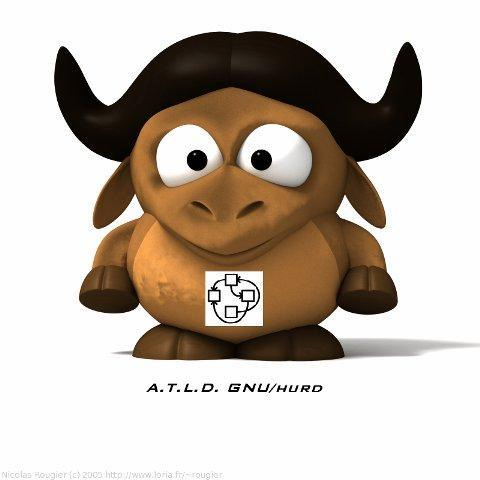
\includegraphics[scale=.4]{images/hurd.png}
        \caption*{GNU/Hurd}
      \end{figure}}

    \visible<2->{\begin{figure}[h!]
        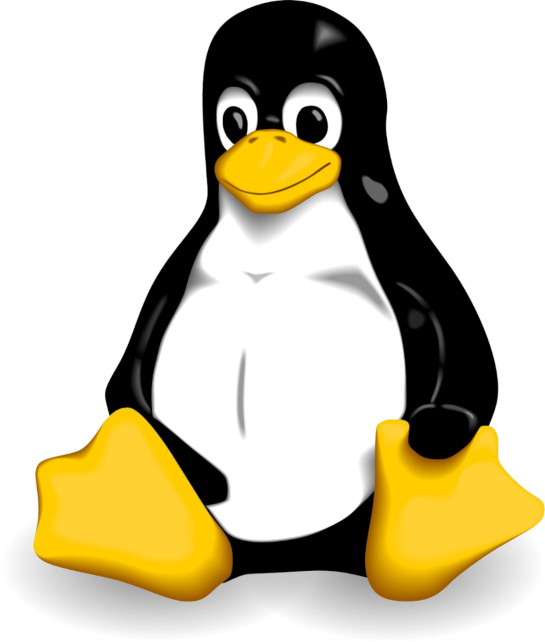
\includegraphics[scale=.25]{images/linux.png}
        \caption*{Linux}
      \end{figure}}

    \visible<3->{\begin{figure}[h!]
        
\includegraphics[scale=.7]{images/freebsd.png}
        \caption*{FreeBSD}
      \end{figure}}

    \visible<4-> {\begin{figure}[h!]
        
\includegraphics[scale=.4]{images/darwin.png}
        \caption*{Darwin}
      \end{figure}}

    \visible<5->{\begin{figure}[h!]
        
\includegraphics[scale=.6]{images/android.png}
        \caption*{Android}
      \end{figure}}
  \end{multicols}
\end{frame}

\subsection{บริษัทที่มีบทบาทในโครงการ FOSS}
% !TeX root = ../.tex
\begin{frame}[t]
  \frametitle{ตัวอย่างบริษัทที่มีบทบาทในโครงการ FOSS}

  \begin{description}[<+->]
    \item[Facebook]  React and React-native JavaScript, Flow, HHVM, Relay
    \item[Google]  Android, Chromium, Dart, Go, Kubernetes, TensorFlow
    \item[Redhat]  OpenShift, Gluster, CloudForms, OpenStack, Fedora, Redhat Linux
    \item[Netflix]  Lipstick, Genie, Inviso, Nebula, Aminator, Spinnaker, Eureka, Aegisthus, Ribbon, Archaius, Hystrix, Governator, Fenzo, Photo, Karyon, Dynomite, Atlas, Chaos Monkey
    \item[Microsoft]  .NET development tools, Visual Studio Code, PowerShell Core, CNTK, Redis, TypeScript
  \end{description}

\end{frame}
% !TeX root = ../.tex
\begin{frame}[t]
  \frametitle{บริษัทที่มีส่วนร่วมในโครงการต่างๆ บน Github}

  \begin{center}
    \begin{figure}[h!]
      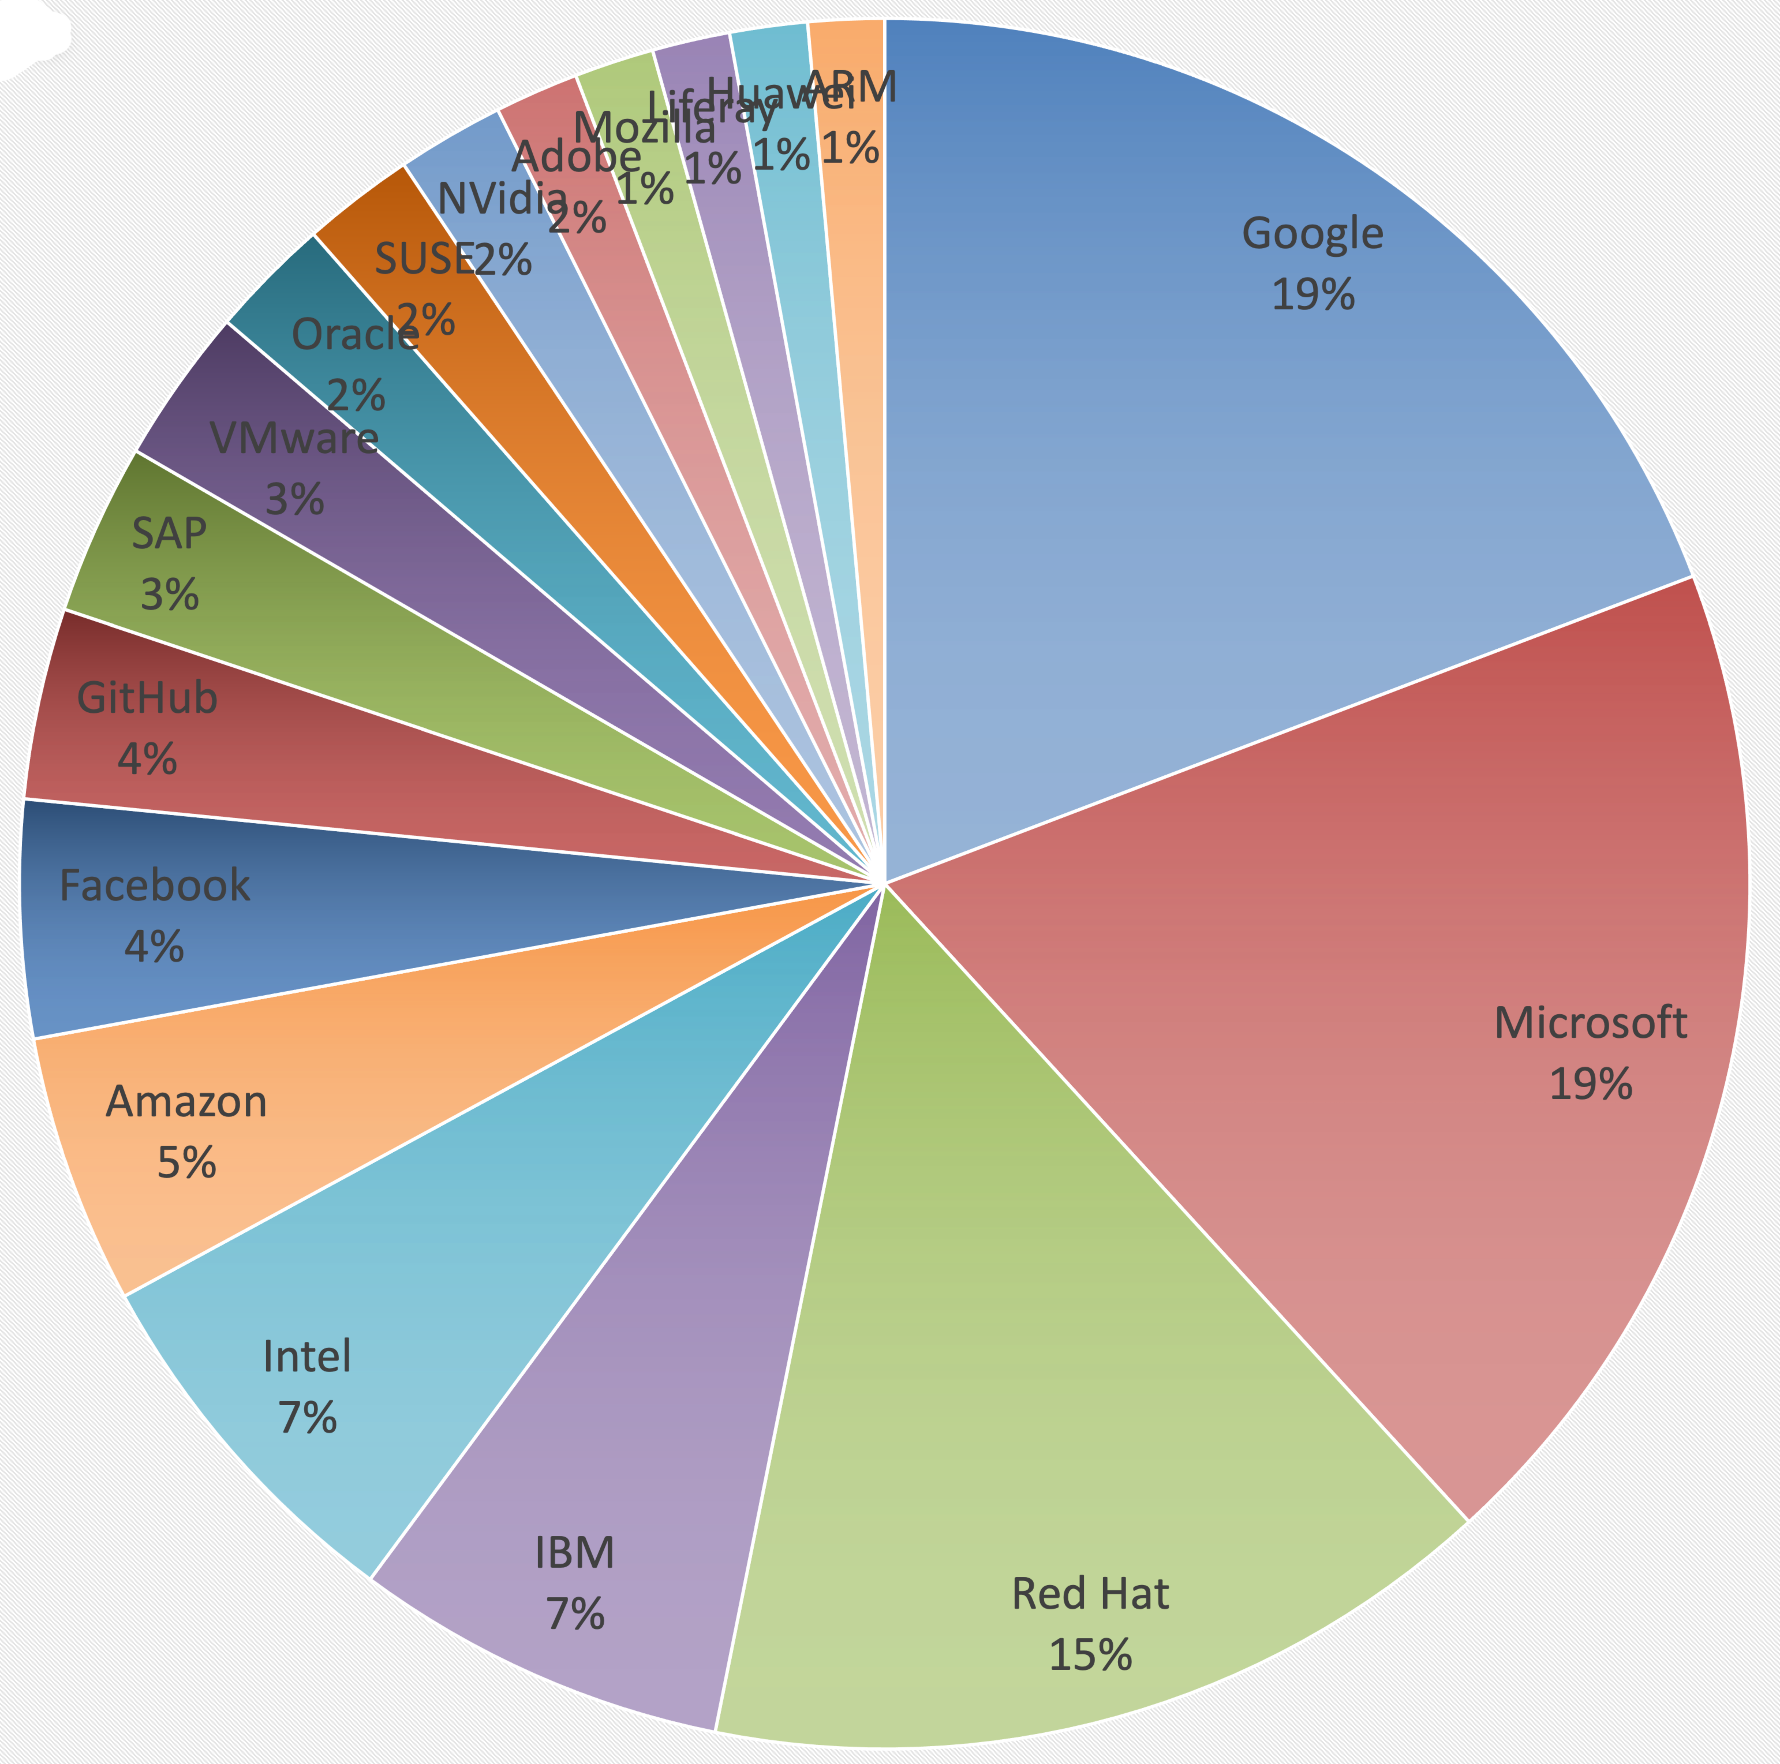
\includegraphics[height=.63\paperheight]{images/github-top.png}
      \caption*{\tiny{Top Contributors on Github} \footnotemark[12]}
    \end{figure}
  \end{center}
  \footnotetext[12]{\url{https://github.com/epam/OSCI}}
\end{frame}

\section{เนคเทค กับการใช้ FOSS }
\subsection{ประวัติ}
% !TeX root = ../.tex
\begin{frame}[t]
  \frametitle{เนคเทคกับ FOSS}

  \begin{columns}

    \column[c]{0.6\textwidth}
    \textbf{ในอดีต}
    \begin{itemize}
      \item ห้องปฏิบัติการโอเพ่นซอร์ส
      \item ลินุกซ์ทะเล (LinuxTLE)
      \item ลินุกซ์ซีส (LinuxSIS)
      \item ลินุกซ์เพื่อคอมพิวเตอร์ราคาประหยัด(Computer ICT)
      \item ลินุกซ์เพื่อผู้ประกอบการภายในประเทศ (Ecolonux)
      \item ออฟฟิซทะเล (OfficeTLE)
    \end{itemize}

    \column{0.4\textwidth}
    \begin{center}
      
\includegraphics[width=.4\linewidth]{images/linuxtle.png}

      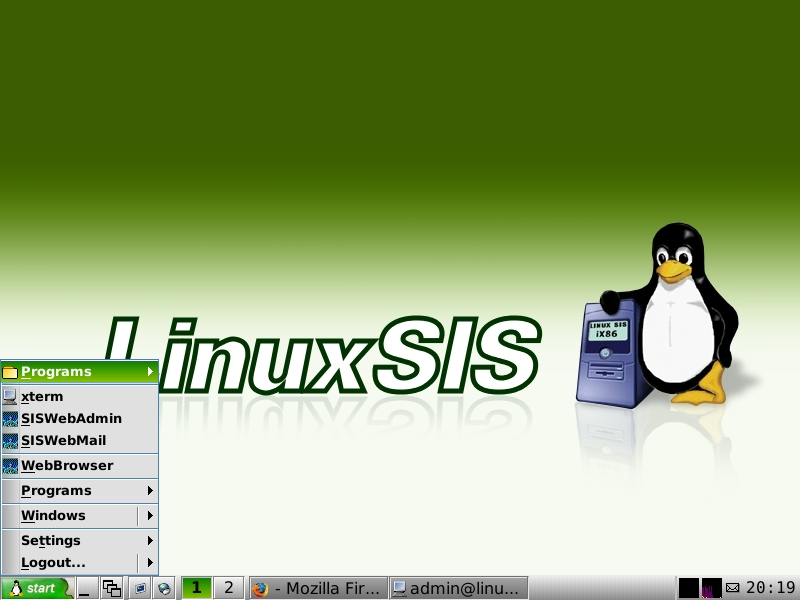
\includegraphics[width=.5\linewidth]{images/linuxsis.jpg}
    \end{center}
  \end{columns}
\end{frame}

\subsection{ปัจจุบัน}
% !TeX root = ../.tex
\begin{frame} [t]
  \frametitle{เนคเทคกับ FOSS}

  \begin{itemize}
    \item การใช้ FOSS สำหรับงานวิจัย
          \begin{itemize}
            \item  ระบบปฎิบัติการ - Linux
            \item ภาษาคอมพิวเตอร์ - Python, GoLang, TypeScript, R
            \item เครื่องมือและไลบรารี่ - TensorFlow, PyTorch, NumPy, Jupyter, SciPy
            \item Plateform และ Microserive - Docker, k8s, HPC (TARA)
          \end{itemize}
    \item การใช้ FOSS เพื่อสร้าง Service Plateform
          \begin{itemize}
            \item  ระบบปฎิบัติการ - Linux
            \item ภาษาคอมพิวเตอร์ - Python, GoLang, TypeScript, R
            \item เครื่องมือและไลบรารี่ - TensorFlow, PyTorch, NumPy, Jupyter, SciPy
            \item Plateform และ Microserive - Docker, CKAN, NGINX, Apache
            \item Analytic Plateform - Elasticsearch,Kibana, Grafana
          \end{itemize}
  \end{itemize}

\end{frame}

\section*{Thank You}
\subsection*{END}
% !TeX root = ../.tex
\begin{frame}
  \frametitle{ขอบคุณ}

  \begin{center}
    {\bfseries \LARGE ขอบคุณครับ}

    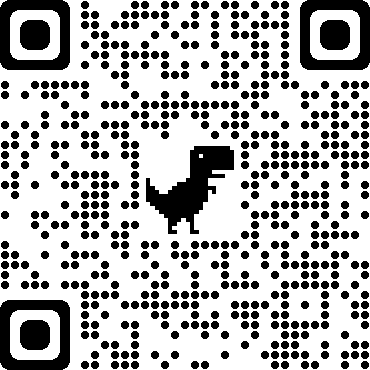
\includegraphics[width=.25\linewidth]{images/qrcode-url.png}


    {\url{https://github.com/mrchoke/presentations/}}
  \end{center}

\end{frame}

\end{document}